\section{Tugas 1 -- Estimasi Waktu Kirim (Regresi P50 dan P90)}
Data latih berisi 250.000 paket yang diambil kurir Januari--Agustus 2025; data uji 60.000 paket September--Oktober 2025.
Target \texttt{durasi\_jam} diprediksi sebagai P50 dan P90 pada saat paket diambil kurir.

\subsection*{(a) Audit data}
\textbf{Kesalahan satuan pada target.} Sebanyak \TsatuDurasiEkstremN{} paket (\TsatuDurasiEkstremPersen\%) memiliki durasi di atas 500 jam
(maksimum \TsatuDurasiMaks{} jam). Jika dibagi 60, median kelompok ini menjadi \TsatuMedianEkstremBagi{} jam, hampir sama dengan median
data normal (\TsatuMedianNormal{} jam) --- bukti kuat bahwa nilai tersebut tercatat dalam menit (Gambar~\ref{fig:t1durasi}).
Tiga perlakuan dibandingkan pada validasi waktu (Tabel~\ref{tab:t1_audit_target}); perlakuan ``dibagi 60'' dipakai.

\textbf{Nilai tidak valid.} \texttt{jarak\_km} bernilai sentinel 9999 (\TsatuJarakSentinelPersen\%) dan 0 (\TsatuJarakNolPersen\%),
juga muncul di data uji, sehingga diubah menjadi \textit{missing} dengan indikator \texttt{jarak\_tidak\_valid}.
\texttt{berat\_kg} kosong pada \TsatuBeratNAPersen\% baris; dibiarkan \textit{missing} (ditangani LightGBM) ditambah indikator.

\textbf{Fitur yang tidak tersedia saat pickup.} Setiap fitur numerik dibandingkan distribusinya antara data latih dan uji (statistik KS)
serta korelasinya dengan target (Tabel~\ref{tab:t1_audit_ks}). \texttt{jumlah\_scan} menonjol: korelasi Spearman dengan durasi
\TsatuScanSpearman{}, tetapi rata-ratanya \TsatuScanMeanTrain{} di data latih dan hanya \TsatuScanMeanTest{} di data uji (KS = \TsatuScanKS).
Scan dicatat \emph{selama} perjalanan; pada saat pickup jumlahnya baru 1--2. \texttt{f30} naik lurus setiap bulan (Gambar~\ref{fig:t1bocor}),
sehingga hanya berfungsi sebagai penanda waktu yang tidak dapat diekstrapolasi ke September--Oktober.

\textbf{Dampak.} Dengan \texttt{jumlah\_scan}, pinball P50 validasi tampak membaik dari \TsatuPinbalBersih{} menjadi \TsatuPinbalScan.
Namun ketika nilai \texttt{jumlah\_scan} diganti dengan distribusi seperti di data uji, pinball P50 memburuk menjadi \TsatuPinbalScanTest{}
dan coverage P90 runtuh (Tabel~\ref{tab:t1_audit_dampak}). Kedua fitur dibuang.

\begin{table}[ht]
\centering\small
\resizebox{\ifdim\width>\linewidth\linewidth\else\width\fi}{!}{%
\begin{tabular}{lrrrr}
\toprule
varian & pinball50 & pinball90 & coverage90 & mae \\
\midrule
tanpa fitur bermasalah (dipakai) & 6.853 & 4.349 & 0.875 & 13.706 \\
+ jumlah\_scan (bocor) & 5.399 & 2.917 & 0.874 & 10.798 \\
+ jumlah\_scan (bocor), nilai seperti di test & 10.545 & 12.338 & 0.441 & 21.090 \\
+ f30 (penanda waktu) & 6.852 & 4.357 & 0.873 & 13.704 \\
\bottomrule
\end{tabular}
}
\caption{Dampak fitur bermasalah pada validasi waktu F2 (latih Jan–Jun, val Jul–Agu).}
\label{tab:t1_audit_dampak}
\end{table}

\begin{figure}[ht]\centering
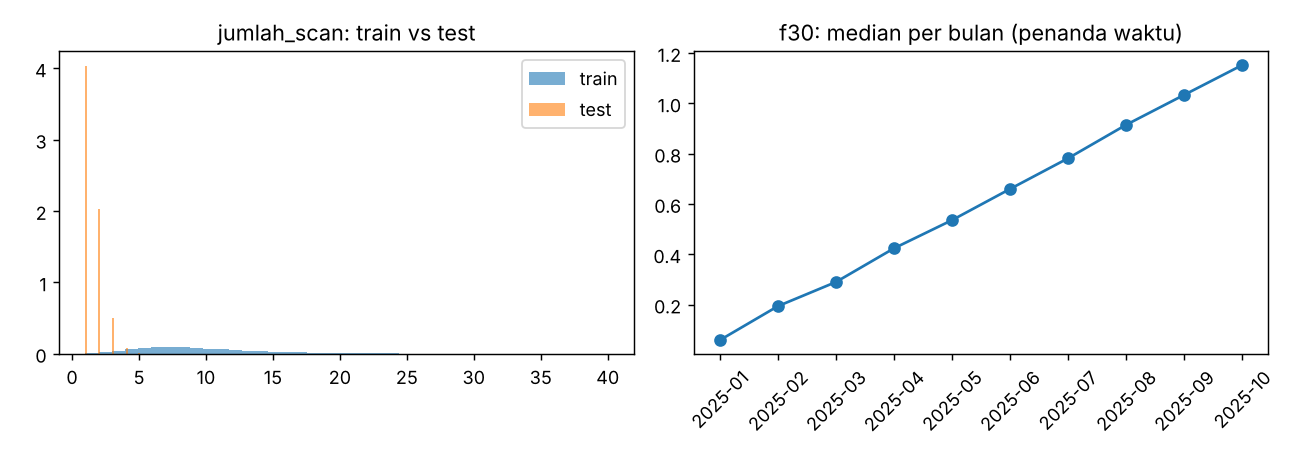
\includegraphics[width=.9\linewidth]{t1_audit_bocor.png}
\caption{Kiri: distribusi \texttt{jumlah\_scan} di data latih vs uji. Kanan: median \texttt{f30} per bulan (penanda waktu).}\label{fig:t1bocor}
\end{figure}

\subsection*{(b) Skema validasi}
Skema utama meniru penggunaan nyata: model dilatih sampai bulan $M$ dan diuji pada dua bulan berikutnya ---
F1 (latih Jan--Apr, uji Mei--Jun) dan F2 (latih Jan--Jun, uji Jul--Agu). Sebagai pembanding, model dan fitur yang sama
dievaluasi dengan random 3-fold CV (Tabel~\ref{tab:t1_validasi}). Random CV memberi pinball P50 rata-rata \TsatuValRandomPinbal{},
lebih optimis dibanding skema waktu (\TsatuValWaktuPinbal), karena model ikut melihat bulan yang sama dengan data uji
(pola musiman dan tren antrean hub). Seluruh tuning dan pemilihan model hanya dilakukan dengan skema waktu.

\begin{table}[ht]
\centering\small
\resizebox{\ifdim\width>\linewidth\linewidth\else\width\fi}{!}{%
\begin{tabular}{llrrrrr}
\toprule
skema & fold & pinball50 & pinball90 & coverage90 & mae & n \\
\midrule
waktu & F1 & 6.795 & 4.216 & 0.906 & 13.590 & 64782 \\
waktu & F2 & 6.853 & 4.349 & 0.875 & 13.706 & 68604 \\
random & R1 & 6.635 & 4.264 & 0.884 & 13.270 & 83334 \\
random & R2 & 6.667 & 4.303 & 0.882 & 13.333 & 83333 \\
random & R3 & 6.631 & 4.242 & 0.882 & 13.263 & 83333 \\
\bottomrule
\end{tabular}
}
\caption{Validasi berbasis waktu vs random 3-fold CV (LightGBM quantile, fitur sama).}
\label{tab:t1_validasi}
\end{table}


\subsection*{(c) Model}
Tiga keluarga model dibandingkan (Tabel~\ref{tab:t1_model}): (i) baseline kuantil empiris per (layanan $\times$ pulau tujuan),
(ii) regresi Ridge dengan target $\log(\text{durasi})$, P90 diperoleh dari kuantil-0,9 residual, dan
(iii) LightGBM dengan \textit{quantile loss} ($\alpha=0{,}5$ dan $\alpha=0{,}9$, dua model terpisah).
Lima konfigurasi LightGBM di-\textit{tune} pada fold waktu (skor = pinball P50 + pinball P90), konfigurasi ke-\TsatuCfgTerbaik{} terbaik.
LightGBM tuned mencapai pinball P50 \TsatuLgbPinbal{} dibanding Ridge \TsatuLinPinbal{} dan baseline \TsatuBasePinbal.

\begin{table}[ht]
\centering\small
\resizebox{\ifdim\width>\linewidth\linewidth\else\width\fi}{!}{%
\begin{tabular}{lrrrr}
\toprule
model & pinball50 & pinball90 & coverage90 & mae \\
\midrule
LightGBM quantile (tuned, cfg 3) & 6.768 & 4.286 & 0.891 & 13.536 \\
LightGBM quantile (default) & 6.824 & 4.282 & 0.890 & 13.648 \\
Linear log-target (Ridge) & 7.417 & 4.571 & 0.913 & 14.834 \\
Baseline kuantil (layanan$\times$pulau) & 10.208 & 6.266 & 0.899 & 20.417 \\
\bottomrule
\end{tabular}
}
\caption{Perbandingan model, rata-rata 2 fold waktu (pinball lebih kecil lebih baik).}
\label{tab:t1_model}
\end{table}


\subsection*{(d) Kategori kardinalitas tinggi dan kategori baru}
\texttt{kota\_tujuan} (405 kategori) dan \texttt{kota\_asal} dibandingkan dengan tiga encoding: target encoding \textit{out-of-fold} dengan smoothing
(dihitung hanya dari data latih fold), frequency encoding, dan kategori native LightGBM (Tabel~\ref{tab:t1_encoding}); terpilih \TsatuKonfigEncoding.
Kategori jarang (< 30 baris) dan kategori yang tidak dikenal dipetakan ke \texttt{\_\_OTHER\_\_}.
Mitra kurir K13 hanya muncul di data uji (±3,9\% baris). Untuk menguji penanganannya, mitra \TsatuMitraSim{} (porsi serupa) dikeluarkan
dari data latih fold F2 lalu diperlakukan sebagai mitra baru (Tabel~\ref{tab:t1_mitra_baru}). Strategi dipilih dengan pinball yang dibobot
porsi mitra baru di data uji; terpilih: \TsatuKonfigMitra.

\begin{table}[ht]
\centering\small
\begin{tabular}{lrrr}
\toprule
encoding kota & pinball50 & pinball90 & coverage90 \\
\midrule
te & 6.832 & 4.356 & 0.874 \\
freq & 6.940 & 4.409 & 0.875 \\
native & 6.845 & 4.385 & 0.873 \\
\bottomrule
\end{tabular}
\caption{Encoding kota\_tujuan/kota\_asal (fold F2).}
\label{tab:t1_encoding}
\end{table}

\begin{table}[ht]
\centering\small
\resizebox{\ifdim\width>\linewidth\linewidth\else\width\fi}{!}{%
\begin{tabular}{lrrrr}
\toprule
strategi & pinball50\_mitra\_baru & coverage90\_mitra\_baru & pinball50\_mitra\_lama & pinball50\_terbobot \\
\midrule
\_\_OTHER\_\_ tanpa dropout & 6.757 & 0.853 & 6.861 & 6.857 \\
\_\_OTHER\_\_ + kategori dropout 5\% & 6.674 & 0.874 & 6.851 & 6.844 \\
tanpa fitur mitra\_kurir & 6.684 & 0.880 & 6.804 & 6.799 \\
\bottomrule
\end{tabular}
}
\caption{Simulasi kategori baru: mitra K12 dikeluarkan dari data latih (fold F2).}
\label{tab:t1_mitra_baru}
\end{table}


\subsection*{(e) Ketidakpastian dan kalibrasi P90}
Model quantile tidak menjamin coverage 90\% bila distribusi bergeser. Kami menerapkan \textit{Conformalized Quantile Regression} (CQR) satu sisi:
skor $s = y - \hat{q}_{0{,}9}$ dihitung pada data \emph{out-of-time}, lalu P90 digeser dengan kuantil-$(1-\alpha)$ skor tersebut.
Kalibrasi dari satu jendela saja ternyata tidak stabil antar fold (Tabel~\ref{tab:t1_kalibrasi}): jendela yang memuat lonjakan Maret membuat koreksi
terlalu besar, sedangkan jendela lain terlalu kecil. Karena itu kami menggabungkan skor dari beberapa jendela bergulir
``latih s.d. bulan $m$, prediksi dua bulan berikutnya'' (horizon yang sama dengan data uji), secara global maupun per layanan (Mondrian).
Pada fold F1 hanya tersedia satu jendela (latih Jan--Feb, kalibrasi Mar--Apr) yang kebetulan memuat lonjakan Maret, sehingga koreksinya
berlebihan --- contoh nyata bahaya kalibrasi dari satu periode. Coverage tanpa kalibrasi juga menurun dari fold ke fold
(Tabel~\ref{tab:t1_kalibrasi}), sehingga risiko \emph{under-coverage} pada September--Oktober nyata.
Aturan pemilihan: dinilai pada fold dengan $\geq 2$ jendela kalibrasi (F2); di antara varian yang pinball P90-nya tidak lebih buruk dari tanpa kalibrasi,
dipilih coverage terdekat 0,90. Pada F2 coverage tanpa kalibrasi \TsatuCovRawFdua{} menjadi \TsatuCovPilihFdua{} dengan varian terpilih
\textbf{\TsatuKonfigKalibrasi}. Gambar~\ref{fig:t1kal} menunjukkan coverage per layanan.

\begin{table}[ht]
\centering\small
\resizebox{\ifdim\width>\linewidth\linewidth\else\width\fi}{!}{%
\begin{tabular}{llrrr}
\toprule
fold & varian & pinball90 & coverage90 & lebar\_median \\
\midrule
F1 & tanpa kalibrasi & 4.216 & 0.907 & 20.941 \\
F1 & CQR jendela terakhir & 4.746 & 0.961 & 34.912 \\
F1 & CQR gabungan lintas bulan & 4.746 & 0.961 & 34.912 \\
F1 & CQR gabungan per layanan & 4.769 & 0.960 & 36.297 \\
F2 & tanpa kalibrasi & 4.356 & 0.874 & 20.017 \\
F2 & CQR jendela terakhir & 4.389 & 0.865 & 18.929 \\
F2 & CQR gabungan lintas bulan & 4.350 & 0.919 & 27.064 \\
F2 & CQR gabungan per layanan & 4.347 & 0.920 & 27.659 \\
\bottomrule
\end{tabular}
}
\caption{Kalibrasi P90 per fold: tanpa kalibrasi, CQR jendela terakhir, CQR gabungan lintas bulan (global / per layanan).}
\label{tab:t1_kalibrasi}
\end{table}

\begin{figure}[ht]\centering
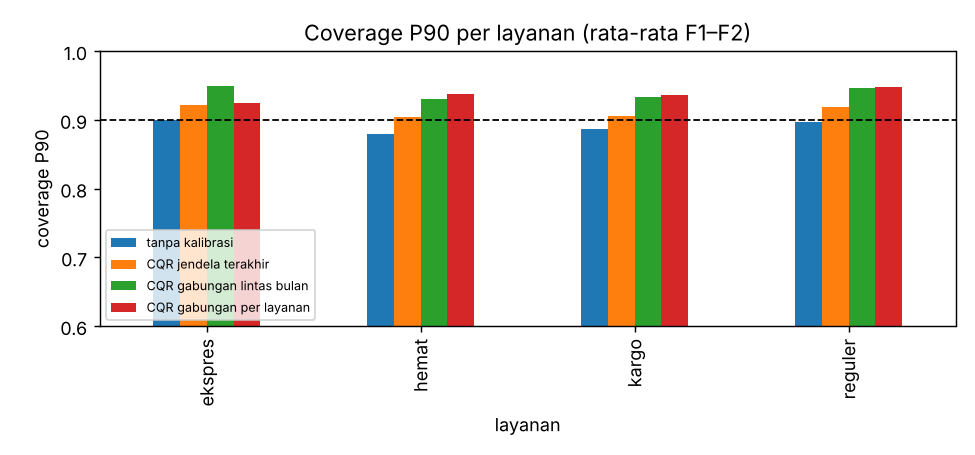
\includegraphics[width=.7\linewidth]{t1_kalibrasi_layanan.png}
\caption{Coverage P90 per layanan untuk tiap varian kalibrasi (rata-rata F1--F2).}\label{fig:t1kal}
\end{figure}

\subsection*{(f) Analisis error dan interpretasi model}
Model final (konfigurasi terpilih + kalibrasi) dievaluasi pada fold F2: pinball P50 \TsatuFinalValPinbal, pinball P90 \TsatuFinalValPinbalNilan,
coverage P90 \TsatuFinalValCov. Error terbesar per layanan terdapat pada \textbf{\TsatuLayananTerburuk} (pinball P50 \TsatuLayananTerburukPinbal),
per pulau tujuan pada \textbf{\TsatuPulauTerburuk} (\TsatuPulauTerburukPinbal), dan per mitra pada \textbf{\TsatuMitraTerburuk} (\TsatuMitraTerburukPinbal)
(Tabel~\ref{tab:t1_breakdown_layanan}--\ref{tab:t1_breakdown_pulau_tujuan}). Error absolut lebih besar pada rute yang durasinya memang panjang;
pola ini konsisten dengan logistik antar-pulau: pengiriman ke Papua (pinball P50 21{,}3 jam) dan Maluku (13{,}8 jam) bergantung pada jadwal kapal atau pesawat yang jarang, sehingga satu jadwal yang terlewat langsung menambah puluhan jam, sedangkan layanan hemat dan kargo lebih sering transit dan menunggu konsolidasi muatan. Mitra K07 perlu perhatian khusus karena coverage P90-nya hanya 0{,}81, jauh di bawah target 0{,}90; artinya model secara sistematis meremehkan durasi mitra ini, sehingga kalibrasi P90 per mitra layak dicoba.
Menurut SHAP (Gambar~\ref{fig:t1shap}), tiga fitur paling berpengaruh pada P50 adalah \texttt{\TsatuShapSatu}, \texttt{\TsatuShapDua}, dan \texttt{\TsatuShapTiga}.
\textit{Partial dependence} (Gambar~\ref{fig:t1pdp}) menunjukkan durasi naik seiring jarak dan antrean hub asal, dengan P90 naik lebih tajam
--- antrean panjang terutama menambah ketidakpastian.

\begin{table}[ht]
\centering\small
\resizebox{\ifdim\width>\linewidth\linewidth\else\width\fi}{!}{%
\begin{tabular}{lrrrrrr}
\toprule
layanan & n & median\_durasi & pinball50 & pinball90 & coverage90 & mae \\
\midrule
hemat & 22760 & 74.500 & 8.706 & 5.065 & 0.915 & 17.412 \\
kargo & 6867 & 79.200 & 7.815 & 4.728 & 0.921 & 15.630 \\
reguler & 28871 & 58.600 & 5.911 & 3.966 & 0.928 & 11.823 \\
ekspres & 10106 & 39.700 & 4.335 & 3.357 & 0.934 & 8.670 \\
\bottomrule
\end{tabular}
}
\caption{Error per layanan (fold F2, model final + kalibrasi).}
\label{tab:t1_breakdown_layanan}
\end{table}

\begin{table}[ht]
\centering\small
\resizebox{\ifdim\width>\linewidth\linewidth\else\width\fi}{!}{%
\begin{tabular}{lrrrrrr}
\toprule
pulau\_tujuan & n & median\_durasi & pinball50 & pinball90 & coverage90 & mae \\
\midrule
Papua & 1226 & 164.050 & 21.304 & 11.220 & 0.888 & 42.608 \\
Maluku & 1341 & 116.500 & 13.759 & 7.037 & 0.915 & 27.518 \\
Kalimantan & 3868 & 92.500 & 11.097 & 6.300 & 0.898 & 22.193 \\
Sulawesi & 4532 & 89.400 & 10.539 & 5.835 & 0.905 & 21.078 \\
Bali-Nusa Tenggara & 2659 & 66.500 & 7.811 & 4.724 & 0.926 & 15.623 \\
Sumatera & 9178 & 64.200 & 7.246 & 4.511 & 0.926 & 14.492 \\
Jawa & 45800 & 56.700 & 5.322 & 3.673 & 0.929 & 10.645 \\
\bottomrule
\end{tabular}
}
\caption{Error per pulau\_tujuan (fold F2, model final + kalibrasi).}
\label{tab:t1_breakdown_pulau_tujuan}
\end{table}

\begin{figure}[ht]\centering
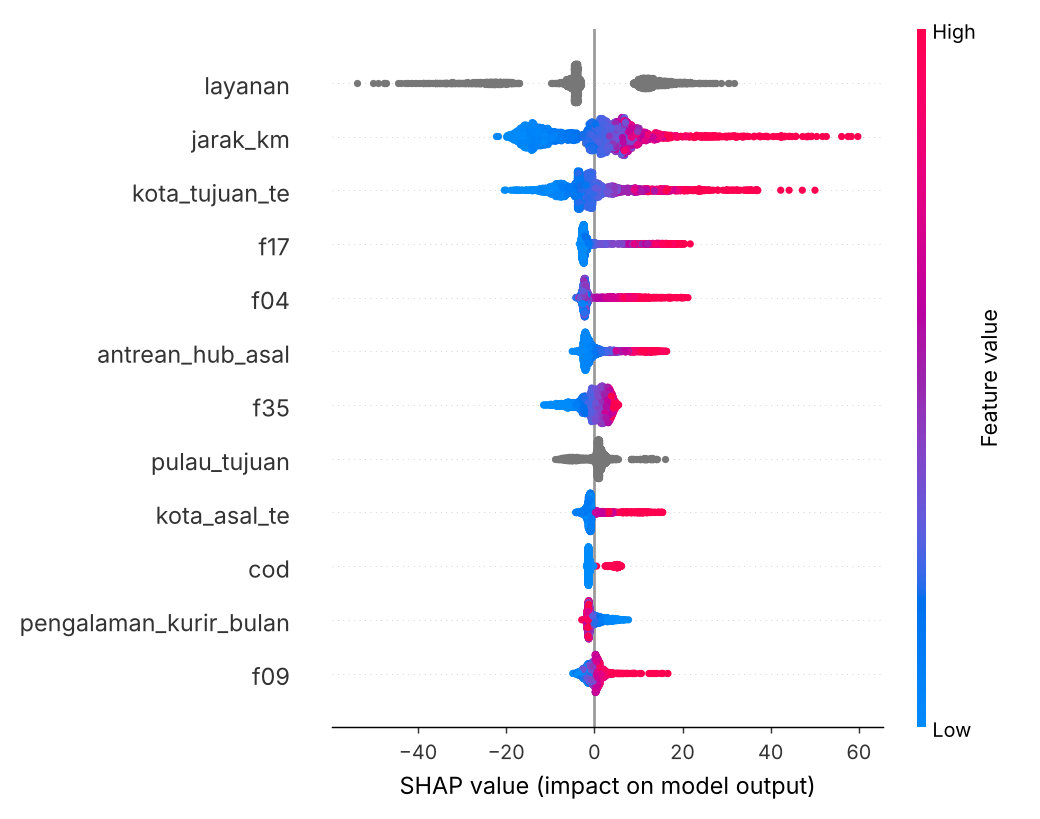
\includegraphics[width=.62\linewidth]{t1_shap_summary.png}
\caption{SHAP summary model P50 (3.000 paket validasi F2).}\label{fig:t1shap}
\end{figure}
\begin{figure}[ht]\centering
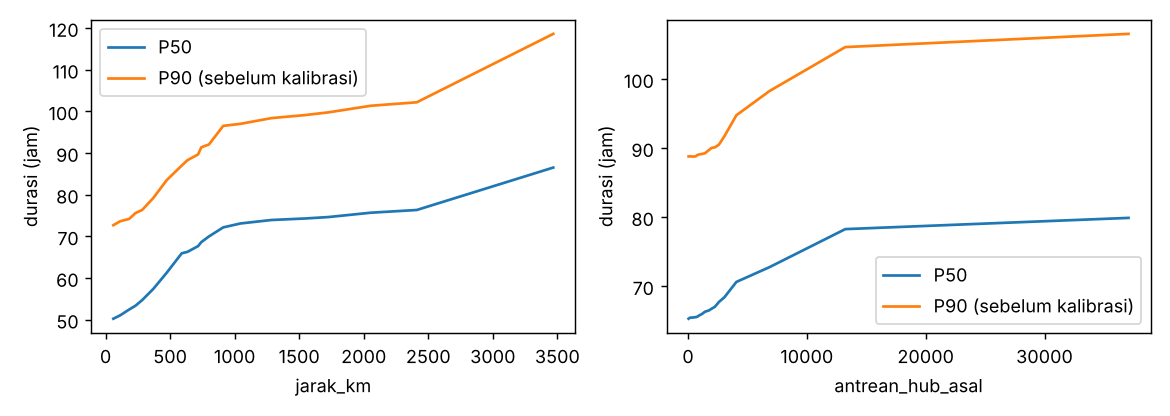
\includegraphics[width=.8\linewidth]{t1_partial_dependence.png}
\caption{Partial dependence P50 dan P90 terhadap jarak dan antrean hub asal.}\label{fig:t1pdp}
\end{figure}

\textbf{Prediksi uji.} Model final dilatih ulang pada Januari--Agustus. Median P50 data uji \TsatuTestPlimaMedian{} jam dan median P90 \TsatuTestPnilanMedian{} jam;
P90 dijamin $\geq$ P50 (koreksi monoton diperlukan pada \TsatuPersenKoreksiMonoton\% paket).
